\subsection{Context and Problem Statement}
\label{problem}

Software development projects for scientific researches are difficult to organise, document and present. There are many examples of the use of software causing the introduction of subtle, but significant issues into scientific research, such as code errors and failures, lack of documentation, false results, and others. 

Python is a programming language that has been developed to be an easy to learn, code and read and has becoming increasingly popular in the scientific programming community for data analysis. Running, testing, debugging and documenting Python scripts has required the usage of various software tools, such as the command prompt (or another command-line interpreter), text editors and others. 

IPython has been created as a software tool, interactive shell for standard scientific Python scripts, that allows combination of styled text, code and data visualizations.\cite{mckinney2012python} It is designed to mimic interactive development environments such as MatLab \cite{matLab} and Maple \cite{maple} for  the writing, testing and debugging of Python code and it has a productive environment for analytical computing. \cite{mckinney2012python} Running Python scripts is effective for immediate response, since developers can see the results right away.

Software can be used in both the development of theoretical models and the analysis of experimental results. Scientific programming is a crucial element of research analysis, since it can give faster and more accurate results - all calculations, models and visualizations can be computed with the help of software tools. As a consequence, scientific programming can be viewed as a another section of conducting researches.\cite{johansson2014introduction} However, researchers are only beginning to understand how software is used in scientific research and the problems encountered when using software.

Scientific programming bring great help and support research, but they have downsides - programming scripts need to be created for a specific area of study, which needs knowledge of both software implementation and the science of the investigated field. Usually analysts are well familiar with only the science that they are doing and as a consequence, they needs to gain computer programming skills. However, programming languages are challenging to learn and a lot of time and practicing is needed for the implementation of the functionality. The analysts might not have the necessary preparation and training in order to create the computations.  

Furthermore, the target readers would probably not be acquainted with the code in the research, so a proper documentation of the software scripts is required - scientists from different areas of studies would be able to understand the code in detail. Thoughts, ideas and findings also need to be recorded for analysis and investigation of the gathered information. Researchers have discover an effective approach for detailing each aspect of a project - handwritten notebooks.\cite{holmes2003reworking} They are commonly used for laboratory experiments. However, researchers have encountered problems with the usage of notebooks - they might not be well organised; each scientist has different style of writing and the reader might have difficulty of reading the notebook; tracking and predicting data with the handwritten notebook is challenging and time-consuming process;

The above problems show that scientists are striving to achieve in reproducible research\textit{" the ability of an entire experiment or study to be duplicated, either by the same researcher or by someone else working independently"}, and replication of results - \textit{"is the repetition of an experimental condition so that the variability associated with the phenomenon can be estimated"}. \cite{reproducibilityWiki} \cite{replicationWiki} They want to be able to produce more shareable document that would give details about the implemented code and the analysis of the findings at the same time. 

IPython Notebook is an open-source projects and they have become an option for scientific researches. The easy set-up and usability is allowing scientists, from different areas of study, to operate with it. It is worth investigating IPython usage in science, since it is an electronic version of the notebooks that researchers have. Also, the main feature of IPython, combining text, code and code output in one file, is of great interest for structuring scientists' ideas and computations. In order to assess the effectiveness of IPython in researches, we have to analyze how is it applied by them and what impact will it have on the problems mentioned above, the issues encountered with the usage of scientific software. 

As a consequence of that, there are specific features of software usage that the project needs to investigate in order to give effective assessment of IPython notebook - e.g. how many GitHub repositories are using IPython for scientific researches, how is it used in a specific area of study, depending on the text and code implemented, what is the proportions of amount of code and the amount of text in the IPython scripts, and others. These questions are illustrating challenges that the project has to confront in order to find the best approach of evaluation of the IPython notebook.  

The \textit{IPython Observatory} project is exploring an explicit environment of researches available for everyone - open source repositories in order to understand the structure and content of IPython notebooks. GitHub, a web-based Git repository hosting service, provides a rich source of IPython source code repositories on the Internet.\cite{gitHubWiki} A huge number of researchers have started to investigate and anlayze GitHub repostories so that they can understand how users are exploiting the site for collaboration on software. \cite{kalliamvakou2007promises} In order to assess the value of IPython in researches, this project will investigate, through analysis of iPython notebooks hosted on Github, how IPython is used in repositories?

\subsection{Proposed Approach}

The project has is analyzing in detail the IPython results from the GitHub search. GitHub is a widely used open source hosting service for projects and, recently, it has become effective place for sharing various researches and contributing to them. It has been chosen for investigation, since it allows tracking of data changes, commits, contributions and documentation. 

The analysis of IPython notebooks on GitHub is broken down to several steps, which are explained in more detail in section \ref{workplan}. Replication and reproducibility of IPython in researches will be the main elements of investigation - they are fundamental for replicating of scientific results. Furthermore, GitHub repositories are important part of projects, as well. The \textit{"The Promises and Perils of Mining GitHub"} is investigating possible threats to the validity of researches involving software projects hosted on GitHub.\cite{kalliamvakoupromises} They can be viewed as fundamental steps for analysing all of the repositories connected with IPython notebooks. Figure \ref{fig:github} is showing the results of the paper. 

\begin{figure}
\centering
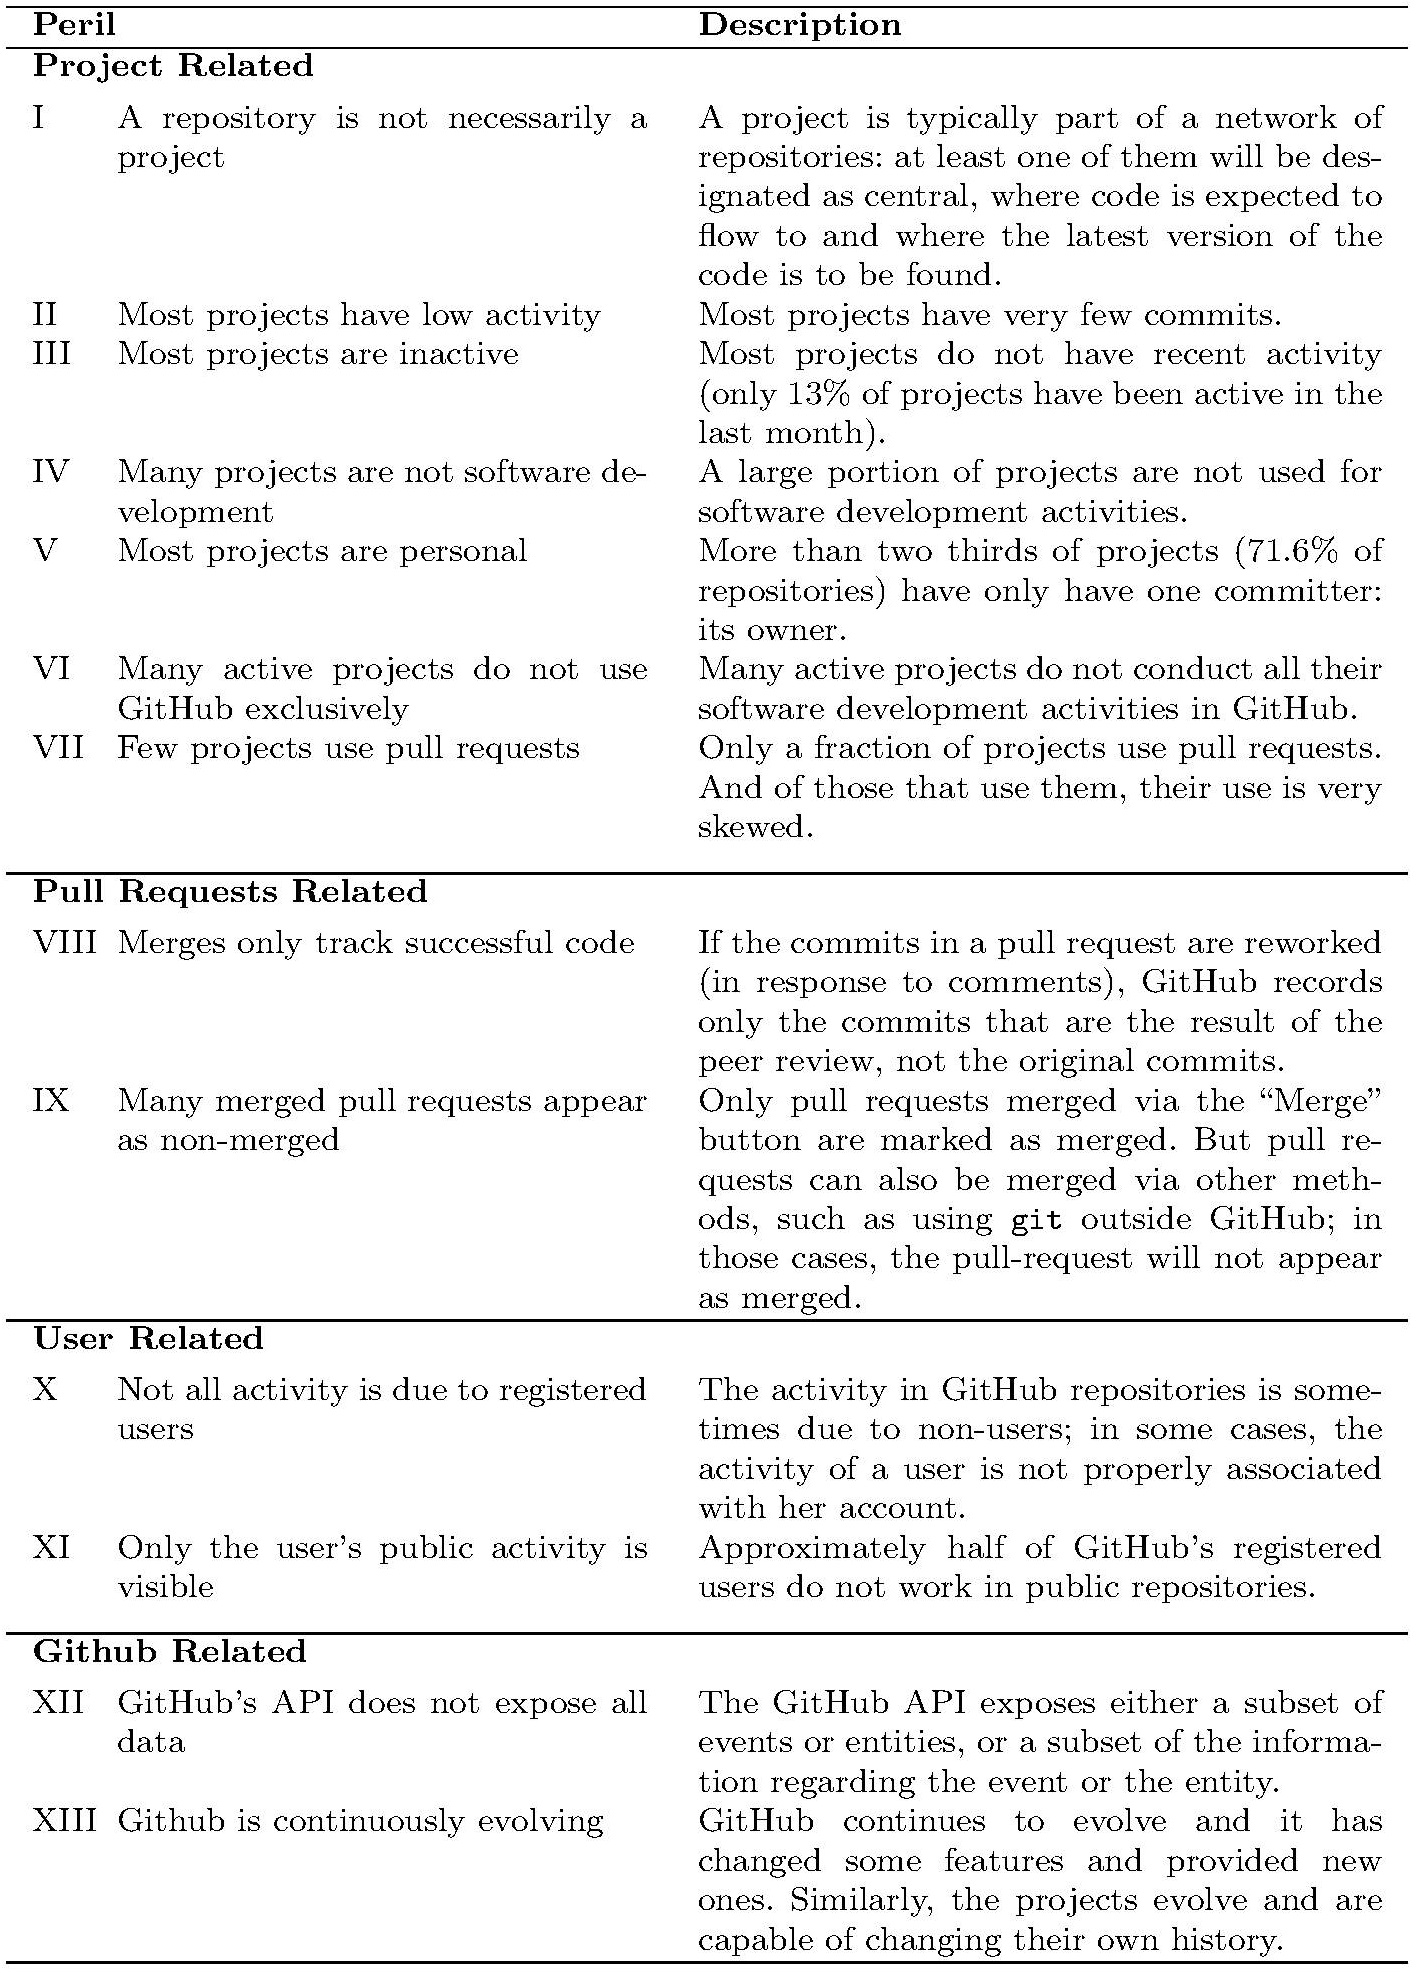
\includegraphics[scale=1.0]{images/file-page1}
\caption{The Promises and Perils of Mining GitHub Results}
\label{fig:github}
\end{figure}

\subsection{Structure of the paper}

Section \ref{problem} of the paper is \textit{"Introduction"}, which gives overview of project's idea, the origins and details of the problem and the paper's structure. In the \textit{"Introduction"} the readers should be able to understand why the usage of IPython notebook is worth analysing.

Section \ref{background} is presenting critical analysis over existing researches - since IPython is a software tool, the reader needs to understand the value of software in scientific researches \ref{softwareSci}, the usage of Python applications \ref{python}, laboratory notebooks \ref{labBooks}, example researches of IPython in scientific programming \ref{IPython} and the data support from open source repositories, such as GitHub \ref{OSS}. 

Section \ref{workplan} is going through the steps of the project - downloading information from GitHub repositories using IPython, analysing GitHub repositories by the aspect from figure \ref{fig:github}, analysing reproducibility and replication of IPython scripts in the downloaded information and their nature of usage - amount of code and text inside them. 

